%!TeX program = xelatex
%Do not change
\documentclass[12pt, oneside]{article}
\usepackage{amssymb,amsmath}
\usepackage[margin=1in]{geometry}
\usepackage{textpos}
\usepackage{float}
\usepackage{booktabs}
%\usepackage{color}
\usepackage{graphicx}
\usepackage[inter-unit-product =\cdot]{siunitx}
\let\DeclareUSUnit\DeclareSIUnit
\let\US\SI
\DeclareUSUnit\inch{in}
\DeclareUSUnit\foot{ft}
\DeclareUSUnit\mile{mi}
\DeclareUSUnit\foot{ft}
\DeclareUSUnit\slug{slug}
\DeclareUSUnit\pound{lb}
\DeclareUSUnit\psi{psi}
\DeclareUSUnit\Msi{Msi}
\DeclareUSUnit\ksi{ksi}

%\usepackage{tikz}
%\usetikzlibrary{positioning}
%\usepackage{tikz-3dplot}
%\usepackage{pgfopts}
%\usepackage{wasysym}
%\usepackage{stanli}

% You may add the packages you need here
\begin{document}

\begin{textblock*}{4cm}(-1.7cm,-2.3cm)
\noindent {\scriptsize AE333 Spring 2021}
\end{textblock*}

%Do not modify other than putting your name where stated
\begin{textblock*}{8cm}(12.5cm,-1cm)
\noindent {Name: }
\end{textblock*}
%Do not modify other than typing your acknowledgement where stated
\begin{textblock*}{13.5cm}(-1.7cm,-1.8cm)
%\noindent \textit{\footnotesize Acknowledgement: Your acknowledgement for collaboration and other sources goes here. }
\end{textblock*}

\vspace{1cm}

%Do not modify other than typing the homework number after #
\begin{center}
\textbf{\Large Homework 2}
\end{center}

\begin{enumerate}
	\item %tension strain problem
		If the load shown causes the point $C$ to displace $\SI{15}{mm}$ find the strain in the ropes $BD$ and $CE$.
		\begin{figure}[H]
			\centering
			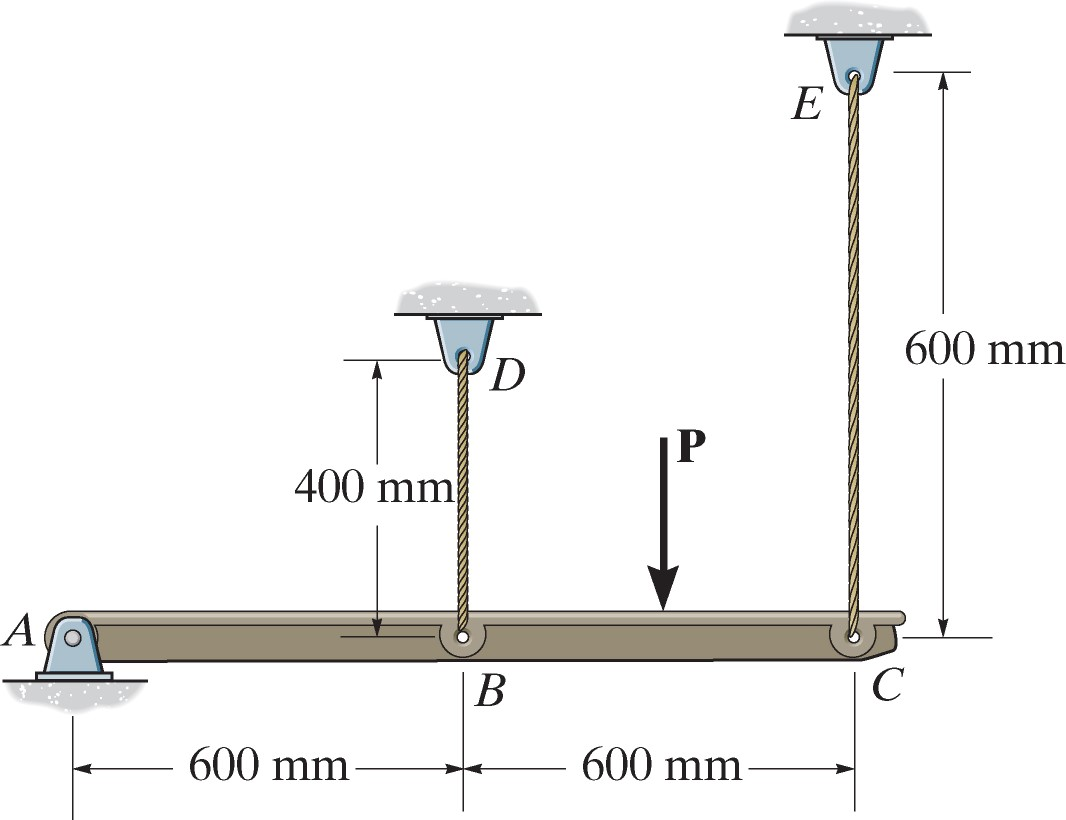
\includegraphics[width=0.5\linewidth]{tension1}
			\label{fig:tension1}
		\end{figure}
		\begin{figure}[H]
			\centering
			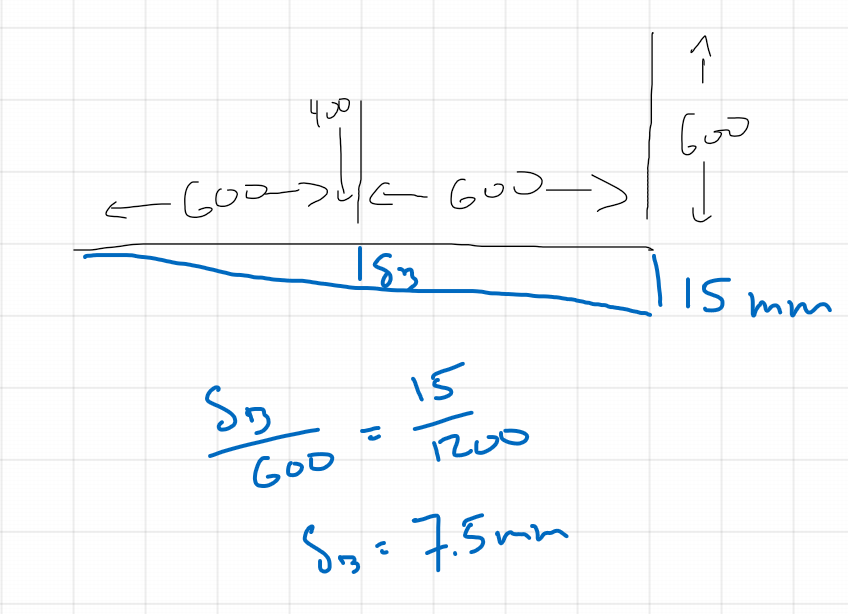
\includegraphics[width=0.5\linewidth]{hw2-1}
		\end{figure}
		\begin{itemize}
			\item We use similar triangles to find the displacement at $B$, $\delta_B = 	\SI{7.5}{mm}$
			\item We can now find the strain in both ropes $\epsilon_{BD} = \frac{7.5}{400} = 0.0188$ and $\epsilon_{CE} = \frac{16}{600} = 0.025$
		\end{itemize}

	\item %tension strain problem
		A flexible cable, $AB$, connects to a rigid member $CB$ as part of an airplane control mechanism.
		A force as shown causes a strain in the cable of $400 \mu \epsilon$, find the angle $\theta$ that the rigid member rotates due to this strain.
		\begin{figure}[H]
			\centering
			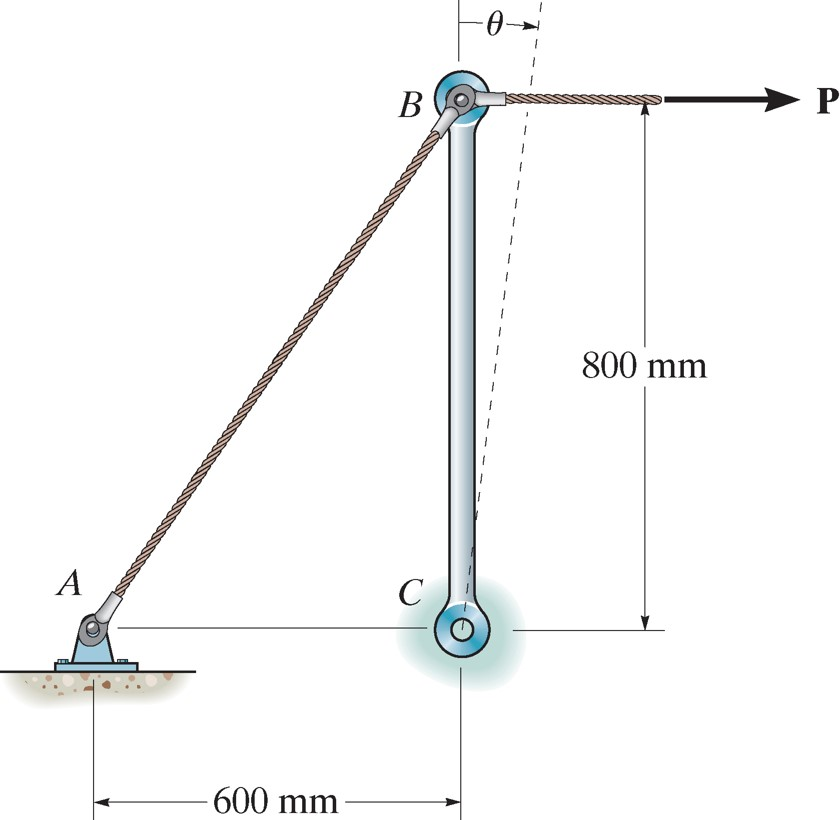
\includegraphics[width=0.5\linewidth]{tension2}
			\label{fig:tension2}
		\end{figure}
		\begin{figure}[H]
			\centering
			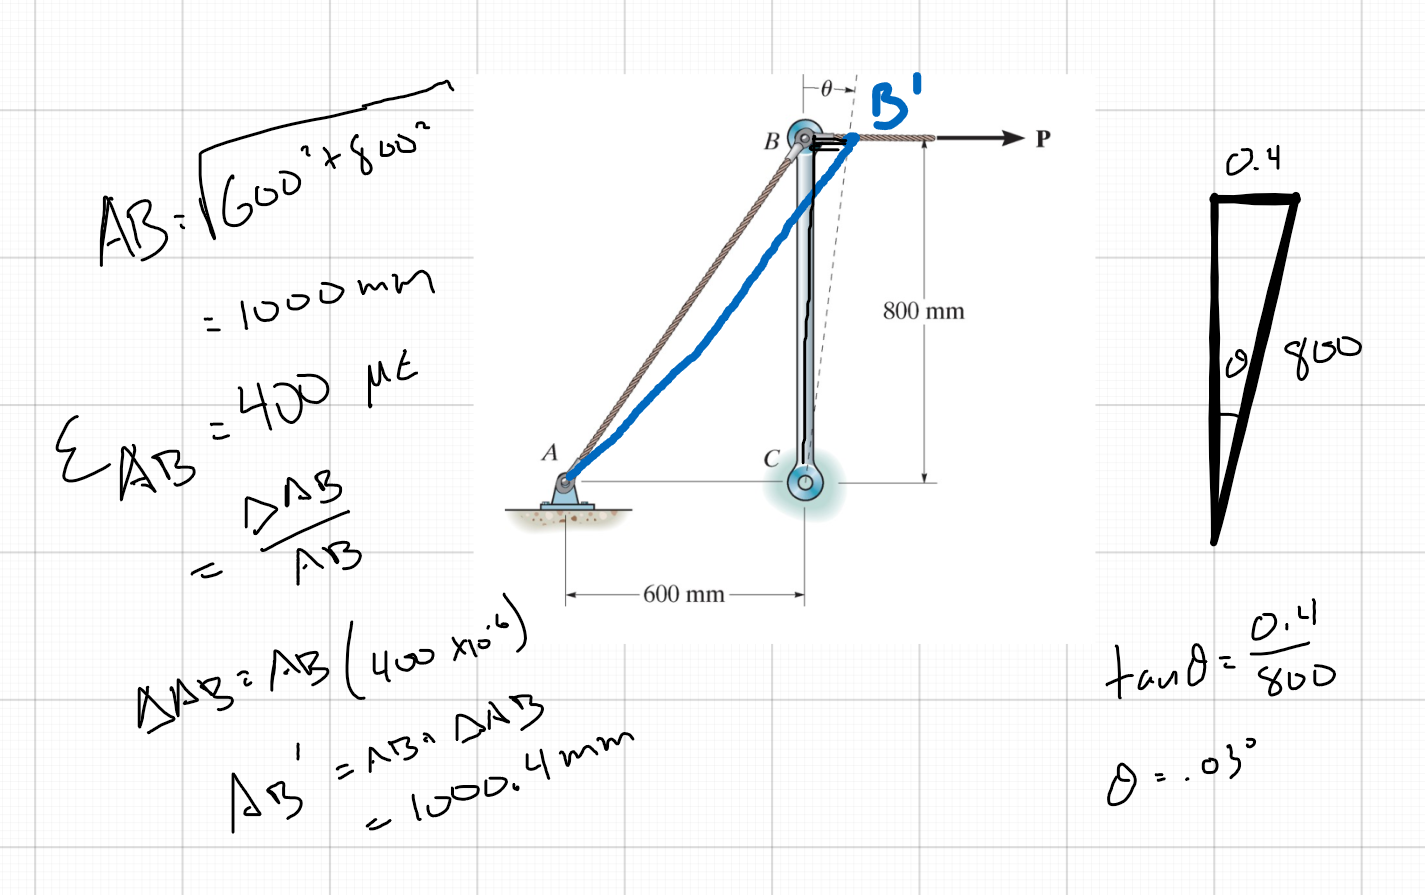
\includegraphics[width=0.6\linewidth]{hw2-2}
		\end{figure}
		\begin{itemize}
			\item We see that $\theta = 0.03^\circ$
		\end{itemize}

	\item %shear strain problem
		Determine the shear strain, $\gamma_{xy}$ at corners $C$ and $D$ for the plate shown.
		\begin{figure}[H]
			\centering
			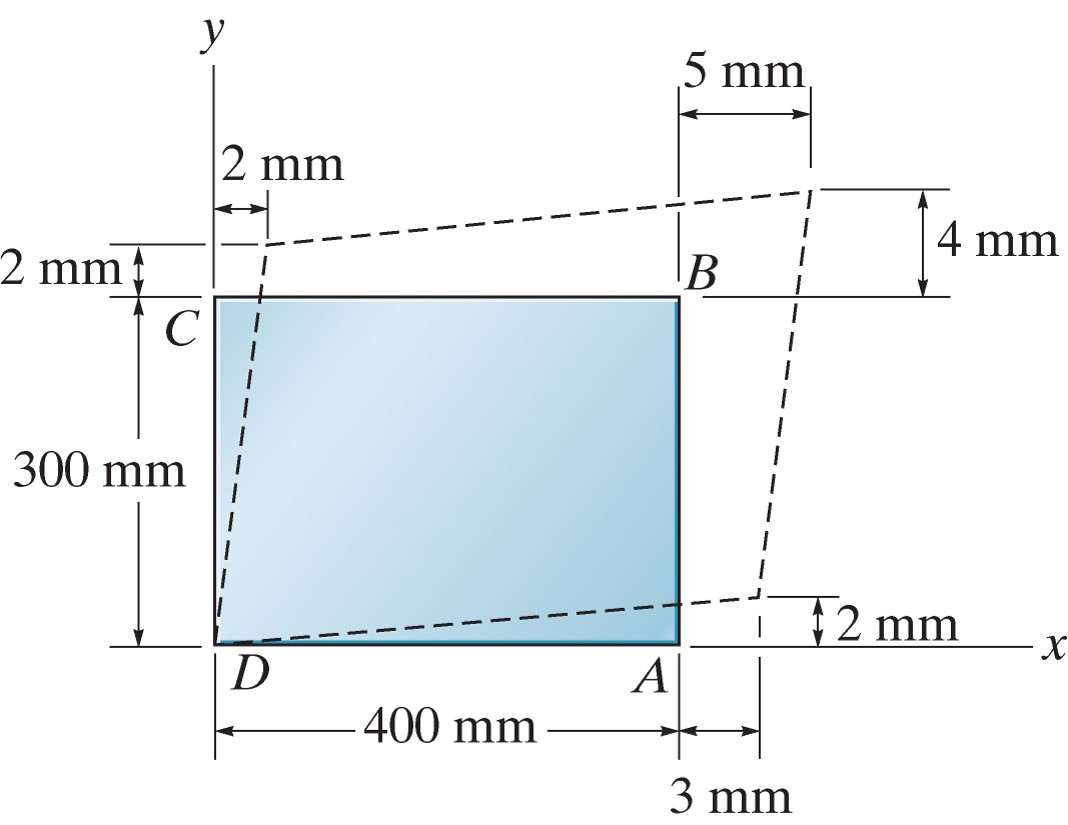
\includegraphics[width=0.5\linewidth]{shear1}
			\label{fig:shear1}
		\end{figure}
		\begin{figure}[H]
			\centering
			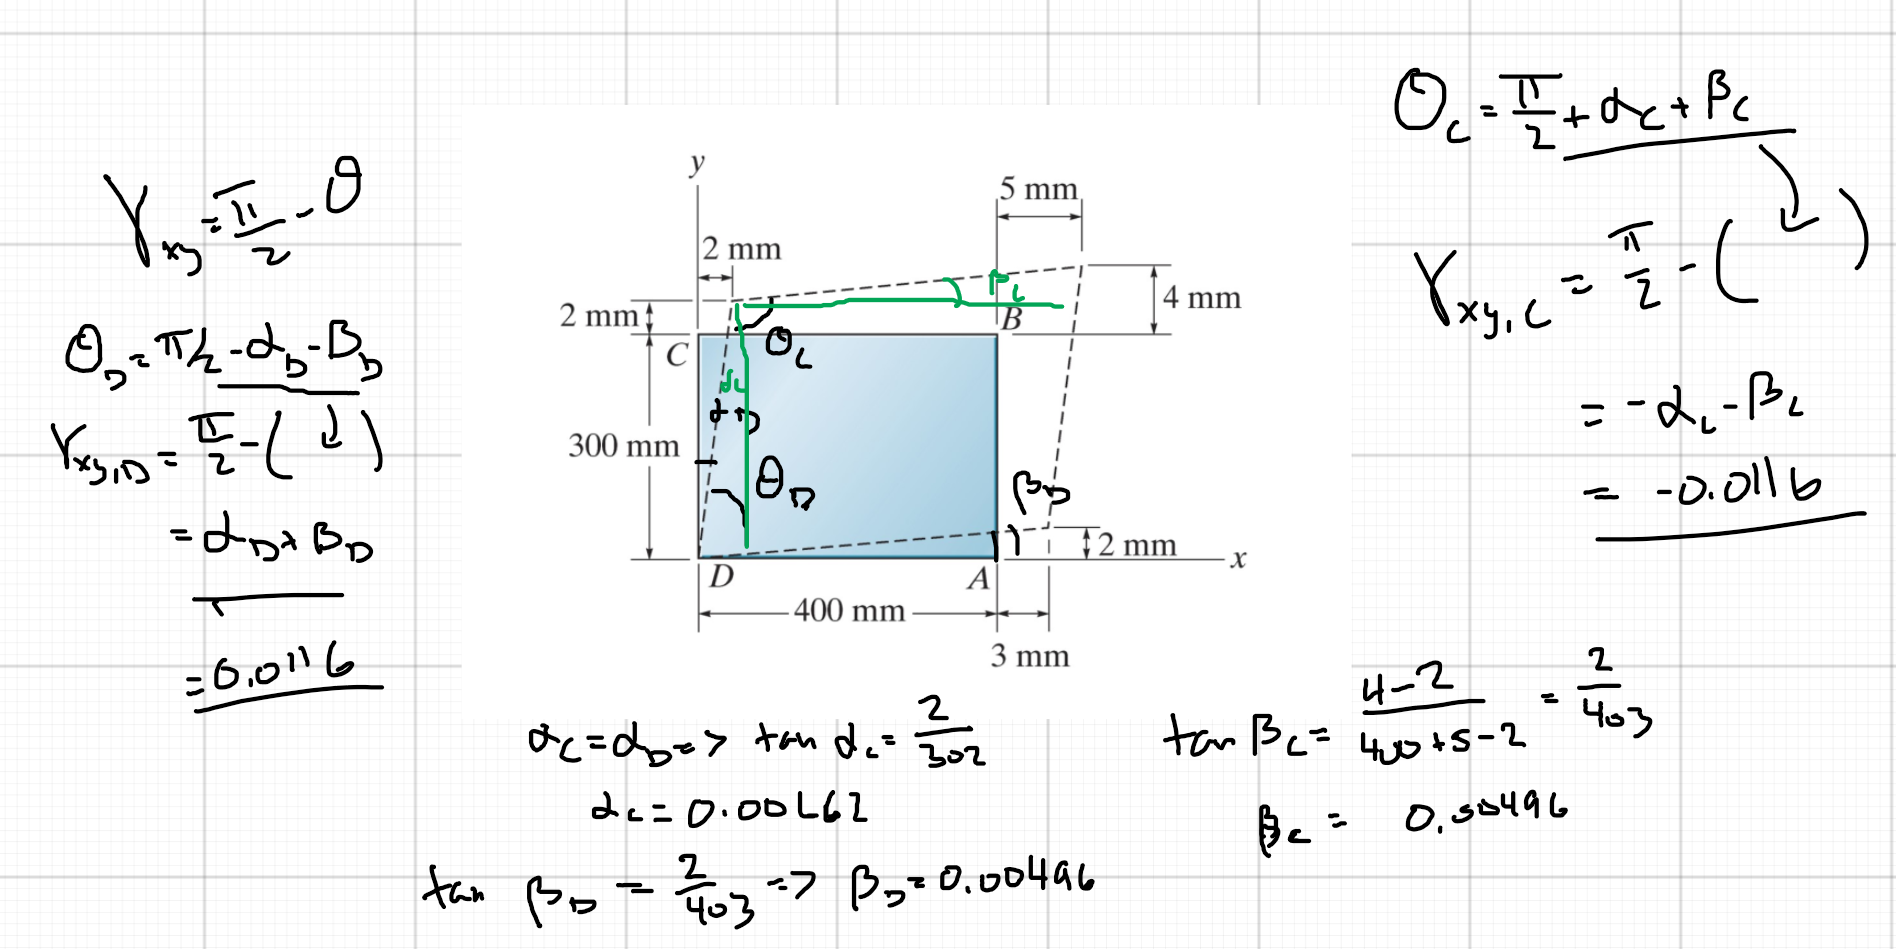
\includegraphics[width=0.7\linewidth]{hw2-3}
		\end{figure}

	\item %shear strain problem
		The polysulfone block is glued at its top and bottom to rigid plates.
		A tangential force applied to the top plate causes the sides to deform so that they are described by the equation $y=3x^{1/3}$.
		Find the shear strain at corners $A$ and $B$.
		\begin{figure}[H]
			\centering
			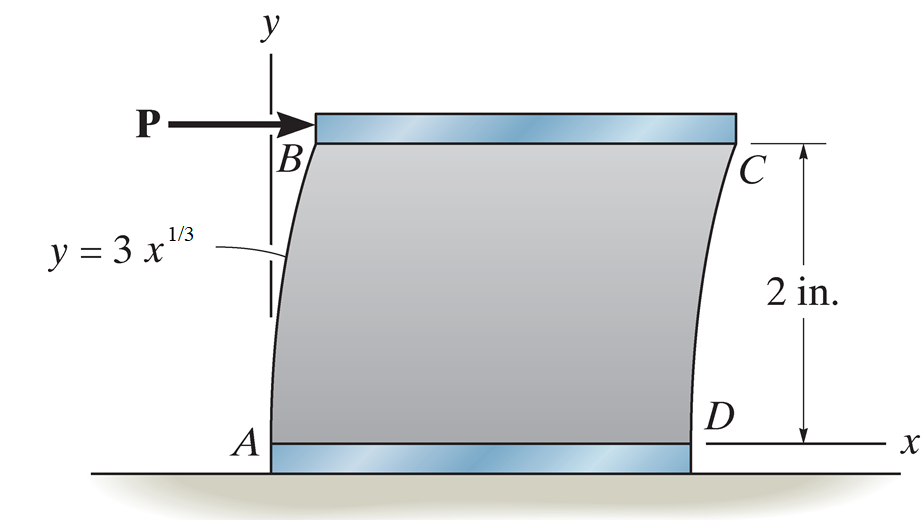
\includegraphics[width=0.5\linewidth]{shear2}
			\label{fig:shear2}
		\end{figure}
		\begin{itemize}
			\item Since we do not have straight lines, for this problem we need to consider the slope of the curved surface at the two points of interest, $A$ and $B$.
			\item We can find these slopes using the derivative
			\item $y^\prime = x^{-2/3}$
			\item The next thing we need to determine is the x-coordinate at $B$ (when $y=2$), we find $x=(2/3)^3 = 0.2963$
			\item Now we can substitute the two known values of $x$ into the derivative, $y^\prime(0) = \infty$, $y^\prime(0.2963) = 2.25$.
			\item The slope at $A$ is infinite, meaning a vertical line, which means $\gamma_{xy,A} = 0$
			\item The slope at $B$ is 2.25, and we can find the associated angle $\gamma_{xy,B} = -0.418$
				\begin{figure}[H]
					\centering
					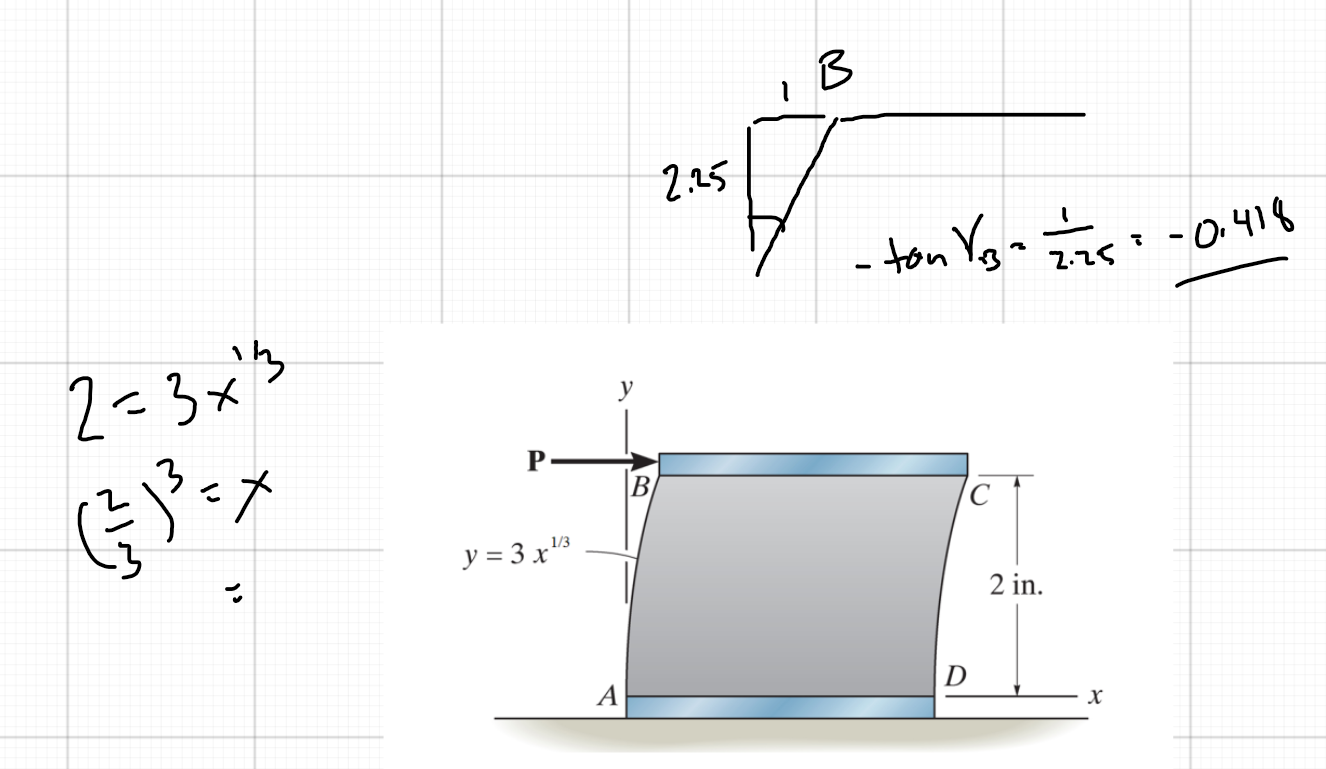
\includegraphics[width=0.6\linewidth]{hw2-4}
				\end{figure}
		\end{itemize}

	\item %elastic mechanical properties
		A tension test was performed on a steel specimen with a cross-sectional area of $\US{0.5}{in^2}$ and a gage length of $\US{2}{in}$.
		Plot the stress-strain diagram and find the modulus of elasticity, the yield stress, and the ultimate tensile strength.
		\begin{table}[H]
			\centering
			\caption{tensile test data}
			\label{tab:label}
			\begin{tabular}{l|l}
				\textbf{Load (kip)} & \textbf{Elongation (in)}\\
				\midrule
				0 & 0\\
				1.50 & 0.0005\\
				4.60 & 0.0015\\ 
				8.00 & 0.0025\\ 
				11.00 & 0.0035\\ 
				11.80 & 0.0050\\ 
				11.80 & 0.0080\\ 
				12.00 & 0.0200\\ 
				16.60 & 0.0400\\
				20.00 & 0.1000\\ 
				21.50 & 0.2800\\ 
				19.50 & 0.4000\\ 
				18.50 & 0.4600\\ 
			\end{tabular}
		\end{table}
		\begin{itemize}
			\item My solution for this problem was performed in Excel, stress and strain were calculated from the load and elongation, then a best-fit line in the linear region was used to find $E$ and $\sigma_Y$, the ultimate tensile strength is the highest stress found.
			\item $E = 	\US{13}{Msi}$, $\sigma_Y = 	\US{23.6}{ksi}$, $\sigma_{ult} = 	\US{43}{ksi} $
			\begin{figure}[H]
				\centering
				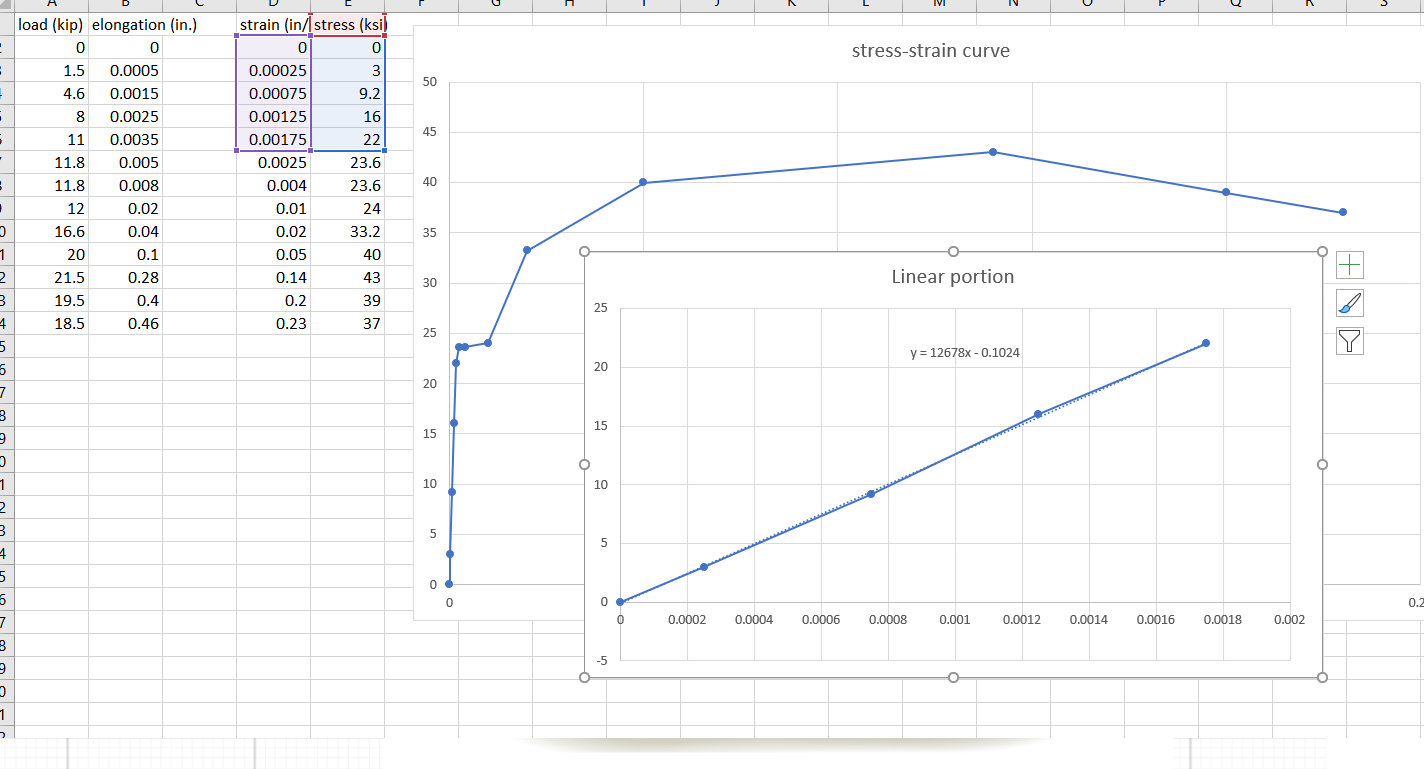
\includegraphics[width=0.7\linewidth]{hw2-5}
			\end{figure}
		\end{itemize}

	\item %elastic mechanical properties
		The rigid beam shown is supported by a pin at $C$ and an A-36 steel wire $AB$.
		If the wire diameter is $\US{0.25}{in}$ determine what the load $w$ is when $B$ is displaced $\US{0.50}{in}$ downward.
		\begin{figure}[H]
			\centering
			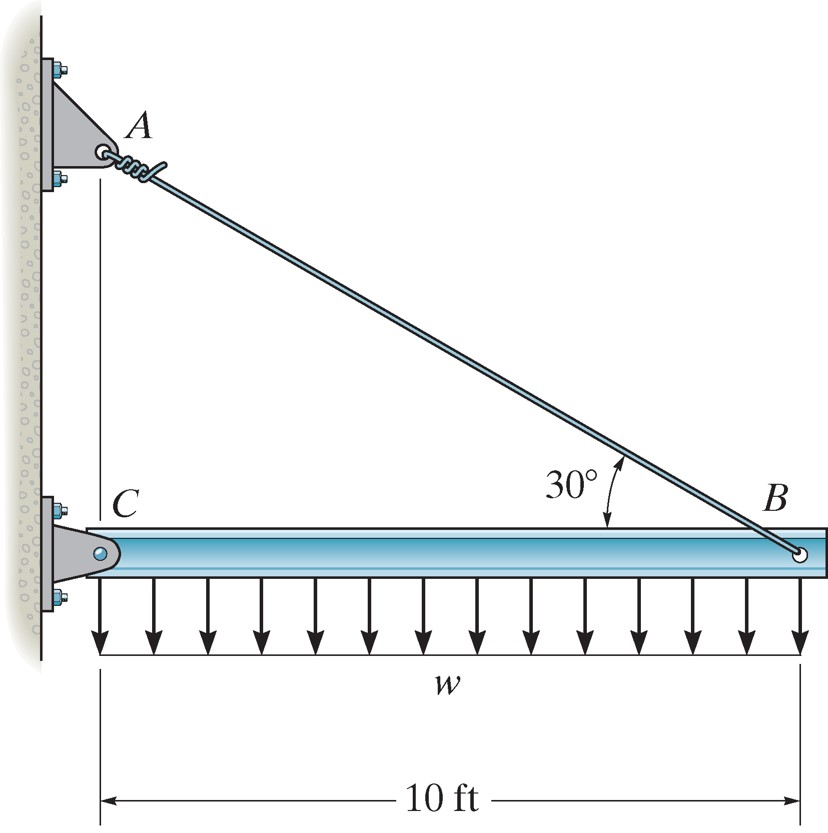
\includegraphics[width=0.5\linewidth]{elastic1}
			\label{fig:elastic1}
		\end{figure}
		\begin{itemize}
			\item Since the beam is "rigid" the displacement at $B$ will be entirely due to stretch of the wire.
			\item We can look up $E$ for A-36 steel in the back cover of the text, $E= 	\US{29.0}{Msi}$
			\item For $\Delta L = \US{0.5}{in}$ we know that $\epsilon = 0.5/12/11.55=0.00361$
			\item Using Hook's Law we know that $\sigma = E\epsilon = \US{29.0}{Msi} .00361$ which gives $\sigma = 	\US{104.6}{ksi}$, which for the given diameter means a force of $ 	\US{5.14}{kip} $
			\item Using statics we can relate the force in the wire to the distributed load
			\begin{figure}[H]
				\centering
				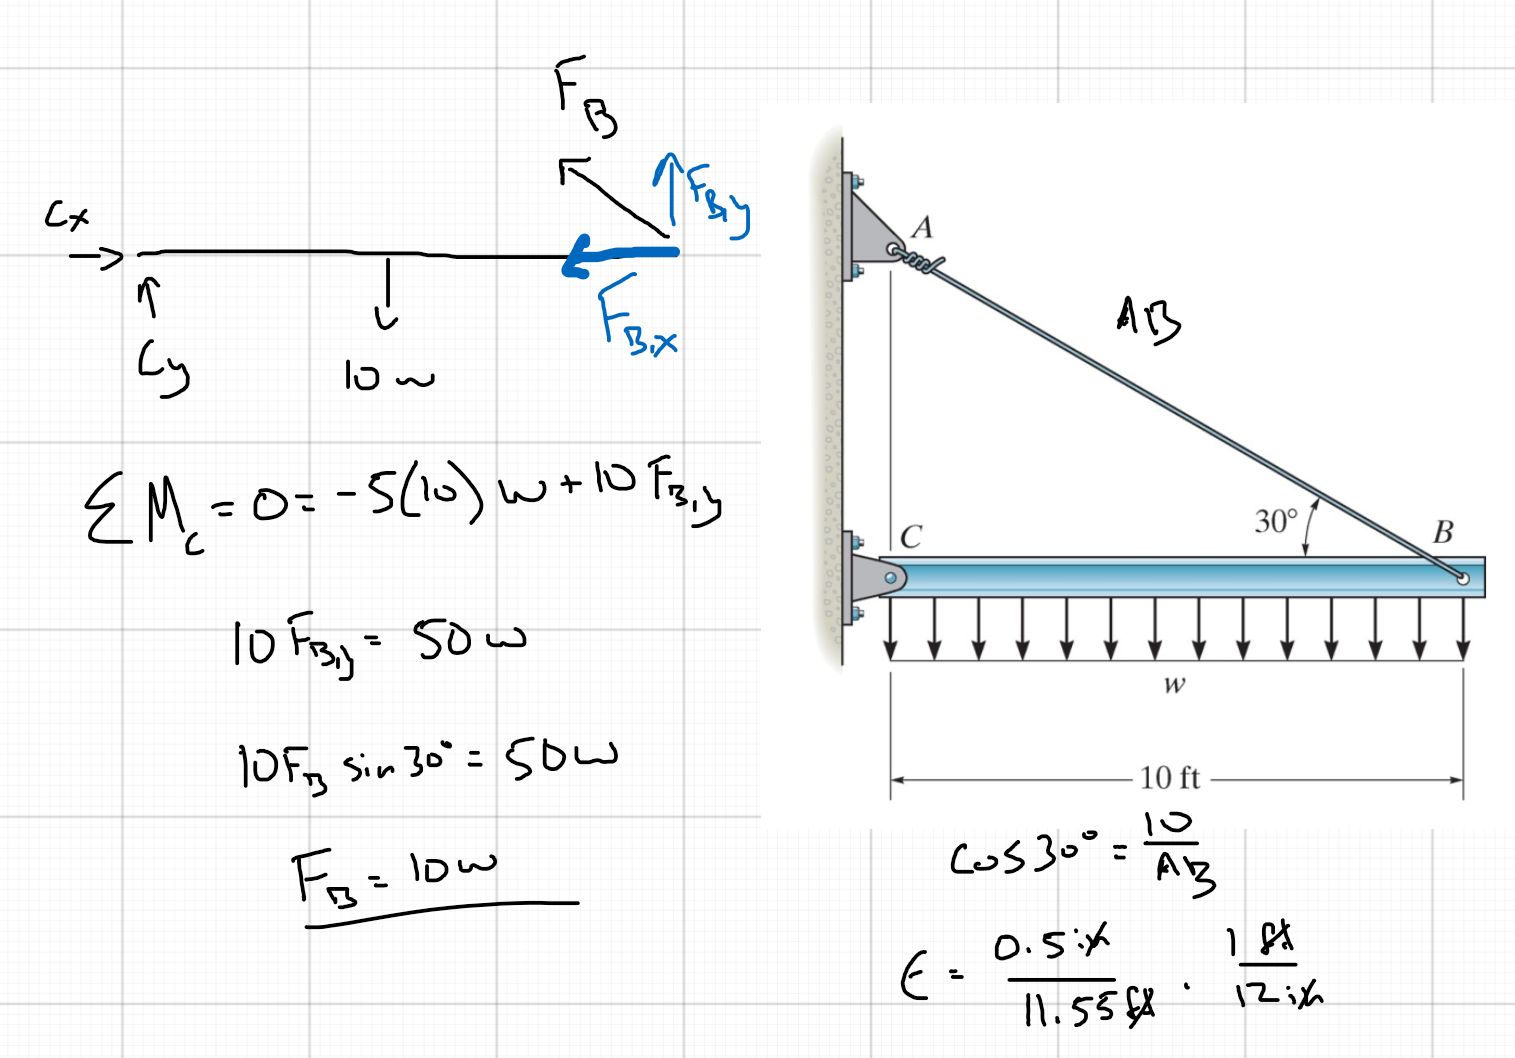
\includegraphics[width=0.6\linewidth]{hw2-6}
			\end{figure}
		\item since $F_B = 	\US{5.14}{kip} = 10w$ we know that $w =	\US{514}{lb/ft} $
		\end{itemize}

	\item %plastic mechanical properties
		The two bars shown are made from the material given in the stress-strain diagram shown.
		Find the cross-sectional area of each bar such that they fail under the same load $P$. 
		Neglect any effects from buckling, consider only tensile and compressive failure.
		\begin{figure}[H]
			\centering
			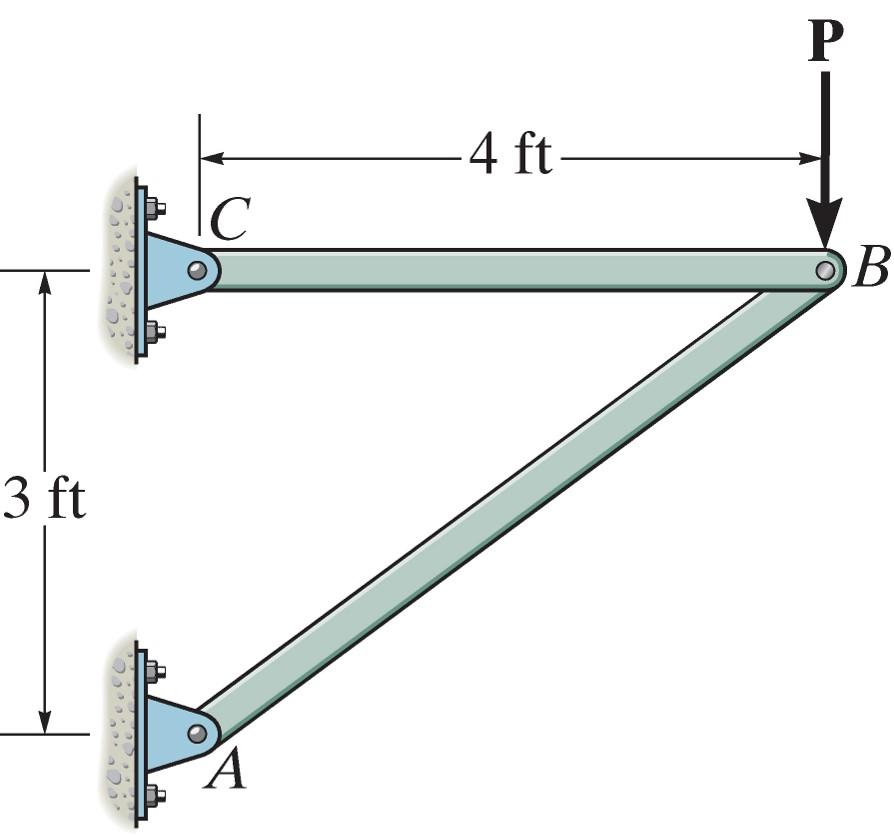
\includegraphics[width=0.4\linewidth]{plastic1}
			\label{fig:plastic1}
		\end{figure}
		\begin{figure}[H]
			\centering
			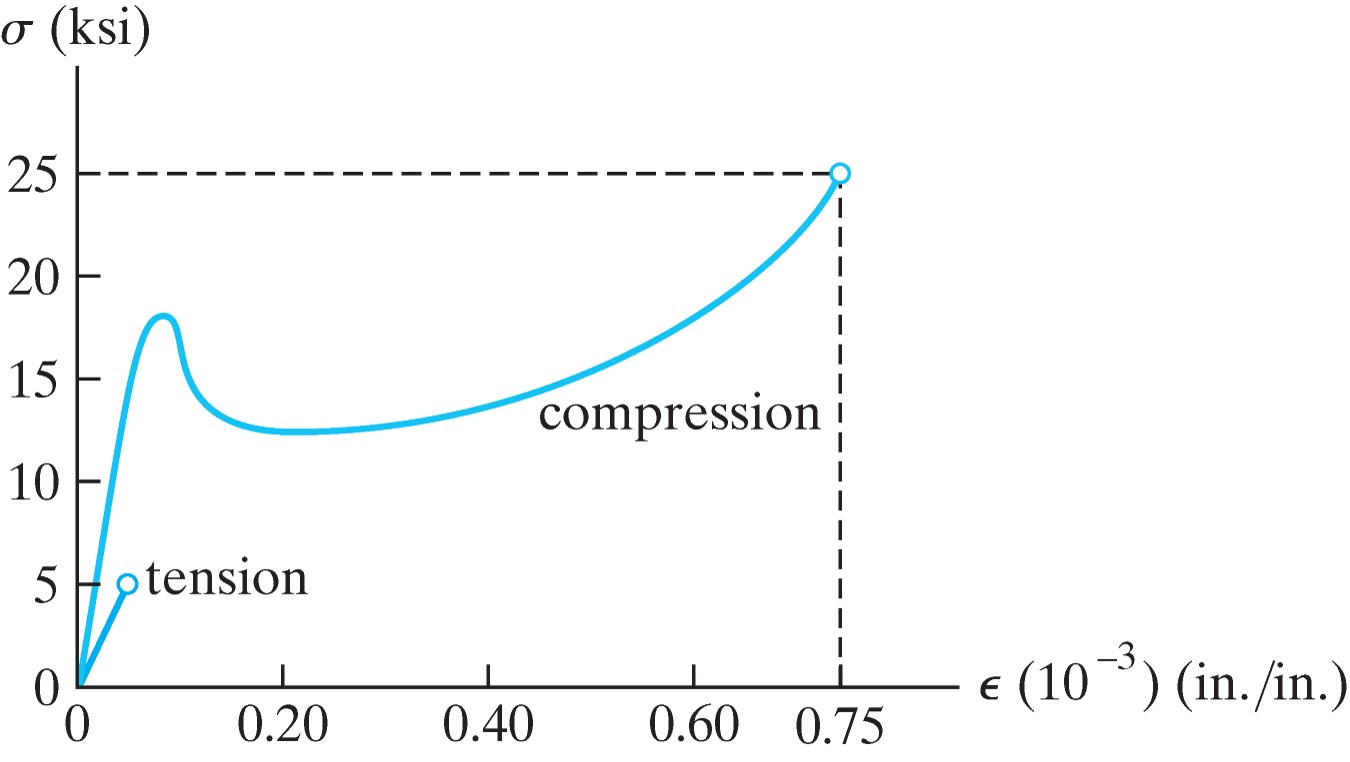
\includegraphics[width=0.7\linewidth]{plastic2}
			\label{fig:plastic2}
		\end{figure}
		\begin{itemize}
			\item We start by doing some statics to determine whether a bar is in tension or compression. Notice that since all forces/reactions occur at pins at the end, these are both 2-force members, so all reaction forces need to act along the axis of the bars
			\begin{figure}[H]
				\centering
				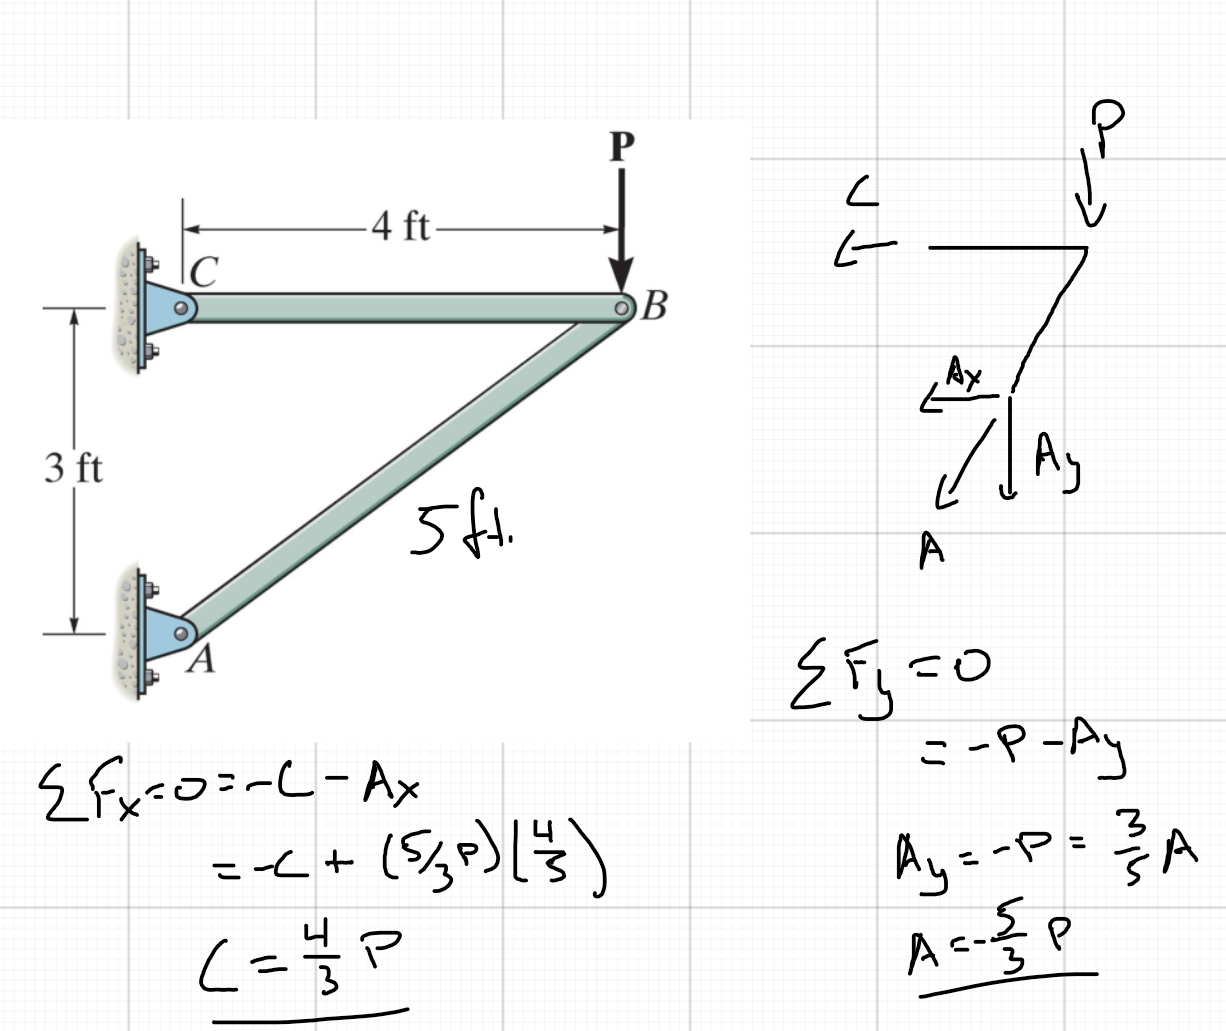
\includegraphics[width=0.6\linewidth]{hw2-7}
			\end{figure}
		\item We see that for a positive $P$ that $AB$ is in compression while $BC$ is in tension. This means that $AB$ will fail at $ 	\US{25}{ksi}  $ and $BC$ will fail at $ 	\US{5}{ksi}  $
		\item We can now find the areas such that the load $P$ will cause failure in both
		\item We will find both areas in terms of the unknown load $P$
		\item $A_{AB} = 5P/3/25 = \frac{1}{15}P$ where $P$ is in k-lb.
		\item $A_{BC} = 4P/3/5 = \frac{4}{15}P$ where $P$ is in k-lb., we see that $BC$ needs an area 4 times the size of $AB$.
		\end{itemize}

	\item %how much strain in rubber band stretched over a rubber band gun
		Dr. Smith made a rubber band gun for his son.
		If the gun is $\US{9}{in}$ long, compare the strain in $\US{0.5}{in}$,  $\US{1}{in}$, and $\US{2}{in}$ diameter rubber bands when stretched over the barrel of the gun.  
		\begin{itemize}
			\item If the rubber bands are perfectly flexible, and we treat them as folding into nearly a straight line, then their initial length is one-half their circumference
			\item The final length will be the length of the rubber band gun, this gives strains of $10.5, 4.7, 1.9$
			\item Rubber deforms much more than most engineering materials (steel, aluminum, wood) and thus has much higher strain values than we are used to seeing
		\end{itemize}

%	\item %delta L for vise screw (compare steel and aluminum)
%		For the leg vise conditions you analyzed in Homework 1, compare the change in length for the vise screw if it were made of steel, aluminum, or wood.

\end{enumerate}
\end{document}
